\begin{frame}{The Tool: Gradient Descent}
    \framesubtitle{The Core Idea}
    \begin{itemize}
        \item We use an iterative optimization algorithm called \bhighlight{gradient descent} to find the minimum of the cost function.
        \item The core idea is to take steps in the direction of the \bhighlight{negative gradient} of the error surface, effectively moving "downhill" to find a minimum.
    \end{itemize}
    \begin{figure}
        \centering
        % Source: Optimization II.pdf, Page: 2
        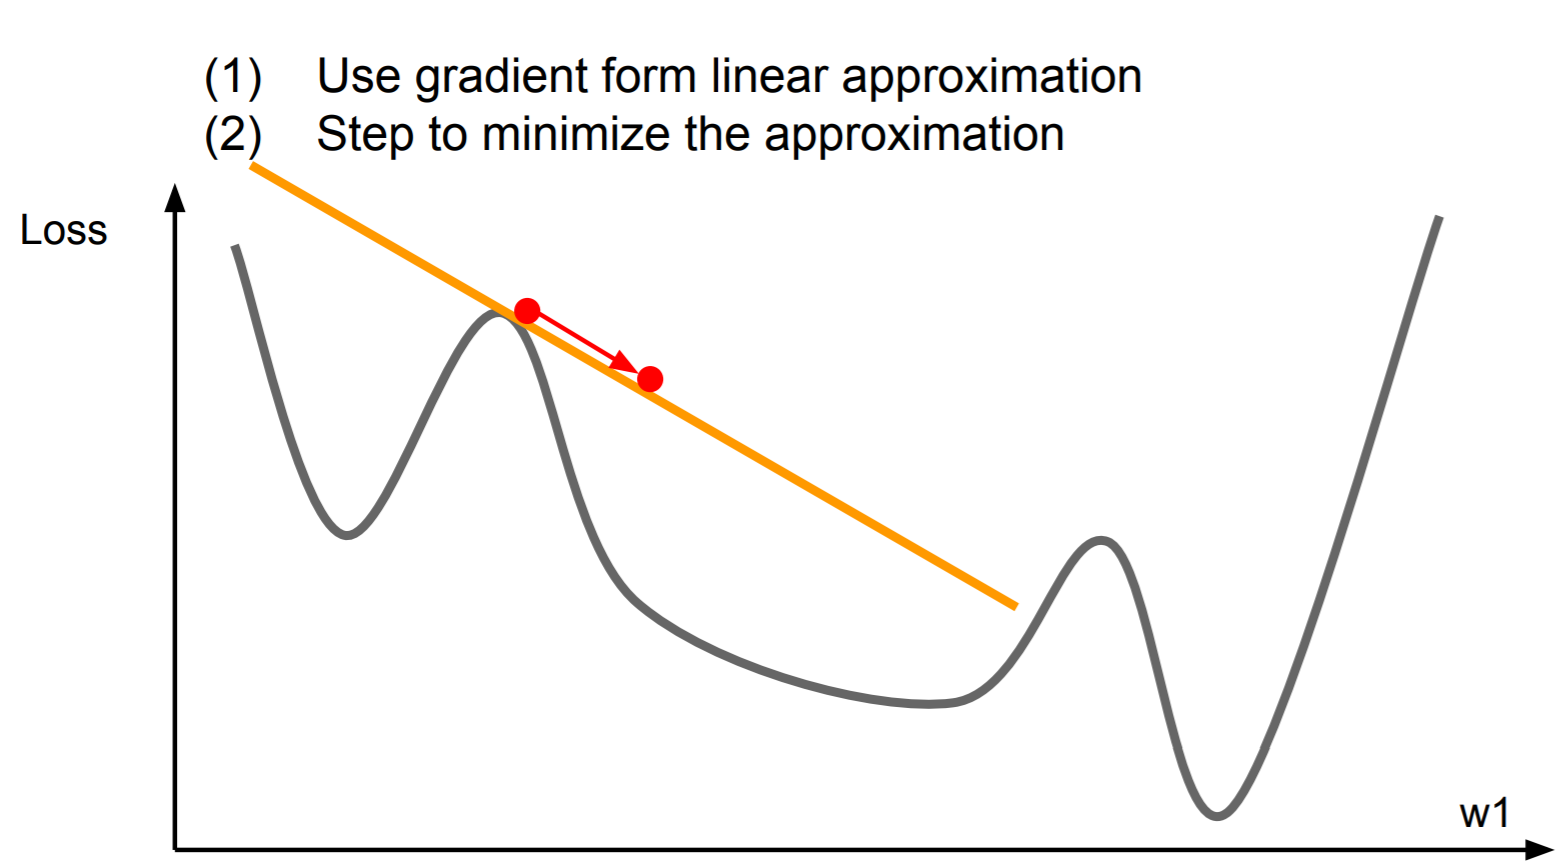
\includegraphics[width=0.7\linewidth]{images/gradient_descent_step.png} 
        \caption{A single step of gradient descent. We form a linear approximation of the loss and step to minimize it.}
    \end{figure}
\end{frame}

\begin{frame}{The Tool: Gradient Descent}
    \framesubtitle{The Update Rule}
    \begin{itemize}
        \item At each step, we update the weights according to the following rule:
        \[
            w^{t+1} = w^{t} - \eta \nabla_{w}J(w^{t})
        \]
        \item Where:
        \begin{itemize}
            \item $w^{t}$ is the vector of weights at step $t$.
            \item $\eta$ (eta) is the \bhighlight{learning rate}, a hyperparameter that controls the step size.
            \item $\nabla_{w}J(w^{t})$ is the gradient of the cost function with respect to the weights.
        \end{itemize}
    \end{itemize}
\end{frame}

\begin{frame}{The Tool: Gradient Descent}
    \framesubtitle{Calculating the Gradient}
    \begin{itemize}
        \item The gradient $\nabla_{w}J$ is computed efficiently using the \bhighlight{backpropagation} algorithm.
        \item Backpropagation is essentially a recursive application of the \bhighlight{chain rule} from calculus to compute the gradient for every parameter in the network.
        \item The process involves two main steps:
        \begin{enumerate}
            \item A \bhighlight{forward pass} to compute the network's output and the final loss.
            \item A \bhighlight{backward pass} to propagate the error gradients from the output layer back to the input layer, calculating the gradient for each weight along the way.
        \end{enumerate}
    \end{itemize}
\end{frame}